\section{Input-selected Cartoon derivative MMS}
\label{sec:cartoon-mms}

\paragraph{Evidence boundary.}
This source describes the frozen manufactured-solution method and the schema that
will consume fresh CPU+MPI and CUDA+MPI evidence.  At this source-review stage no
backend campaign result is claimed.  The final report must be rebuilt from the
checksum-bound accepted JSON/CSV before any numerical table or convergence plot is
presented as a result.

\subsection{Coordinates, fields, and regularity}
The analytic oracle is generated first in conventional Cartesian order $(x,y,z)$,
on the meridional plane $y=0$, and only then permuted to provider order
$(\rho,z,Y)=(x,z,y)$.  With $s=x^2+y^2$, $R^2=s+z^2$, and
$E=\exp(-R^2/5)$, the scalar is
\[
 f=E\left(1+0.17z+0.11s-0.07sz+0.03z^3\right).
\]
Writing $\boldsymbol r=(x,y,0)$, $\boldsymbol\phi=(-y,x,0)$, and
$\boldsymbol e_z=(0,0,1)$, the vector is
$\boldsymbol V=A\boldsymbol r+C\boldsymbol\phi+B\boldsymbol e_z$.
The coefficient functions used by the generated oracle are
\begin{align*}
A&=E(0.70+0.13z+0.09s-0.04z^2),&
B&=E(-0.20+0.19z-0.06s+0.05sz),\\
C&=E(0.30-0.08z+0.07s+0.02z^2).
\end{align*}
Consequently its provider-plane values are
\[
 (V_\rho,V_z,V_Y)=(\rho A,B,\rho C).
\]
For the symmetric tensor, the six stored provider-plane components are
\[
 (T_{\rho\rho},T_{\rho z},T_{\rho Y},T_{zz},T_{zY},T_{YY})
=(P+Q\rho^2,U\rho,H\rho^2,Z,W\rho,P).
Here
\begin{align*}
P&=E(1.10+0.12z+0.05s),&Q&=E(-0.30+0.07z-0.04s+0.02z^2),\\
H&=E(0.21-0.05z+0.03s),&U&=E(-0.17+0.09z+0.02s),\\
W&=E(0.14+0.04z-0.03s),&Z&=E(0.90-0.11z+0.08s-0.02sz).
\end{align*}
\]
The nonzero $C,H,W$ sectors exercise twist.  Under the independent $\pi$ rotation,
provider component signs are $(-,+,-)$, and at the true axis the oracle enforces
$V_\rho=V_Y=T_{\rho z}=T_{zY}=T_{\rho Y}=0$ and
$T_{\rho\rho}=T_{YY}=P$.

\subsection{SO(2) derivative identities}
For $\rho\ne0$, the provider reconstructs suppressed derivatives from the
rotation generator rather than reading a suppressed storage direction.  Core
identities exercised independently by the oracle include
\begin{align*}
\partial_Y f&=0,& \partial_Y^2f&=\rho^{-1}\partial_\rho f,\\
\partial_Y(V_\rho,V_z,V_Y)&=(-V_Y/\rho,0,V_\rho/\rho),\\
\partial_Y(T_{\rho\rho},T_{\rho z},T_{\rho Y},T_{zz},T_{zY},T_{YY})
 &=(-2T_{\rho Y}/\rho,-T_{zY}/\rho,
 (T_{\rho\rho}-T_{YY})/\rho,0,T_{\rho z}/\rho,
 2T_{\rho Y}/\rho).
\end{align*}
Representative second identities are
\begin{align*}
\partial_Y^2V_z&=\rho^{-1}\partial_\rho V_z,&
\partial_Y^2V_{\rho,Y}&=\rho^{-1}\partial_\rho V_{\rho,Y}
                         -\rho^{-2}V_{\rho,Y},\\
\partial_Y^2T_{\rho\rho}&=\rho^{-1}\partial_\rho T_{\rho\rho}
-2\rho^{-2}(T_{\rho\rho}-T_{YY}),&
\partial_Y^2T_{YY}&=\rho^{-1}\partial_\rho T_{YY}
+2\rho^{-2}(T_{\rho\rho}-T_{YY}),\\
\partial_Y^2T_{\rho Y}&=\rho^{-1}\partial_\rho T_{\rho Y}
-4\rho^{-2}T_{\rho Y}.
\end{align*}
Mixed $\rho Y$ and $zY$ identities are obtained by differentiating the first
generator identities and are checked component-by-component.  At $\rho=0$ the
bounded diagnostic provider replaces quotients by their Taylor limits, for example
$\partial_Y^2f=\partial_\rho^2f$ and
$\nabla\!\cdot V=2\partial_\rho V_\rho+\partial_zV_z$.

\subsection{Signed-plane layout}
\begin{figure}[ht]
\centering
\ifmmsplots
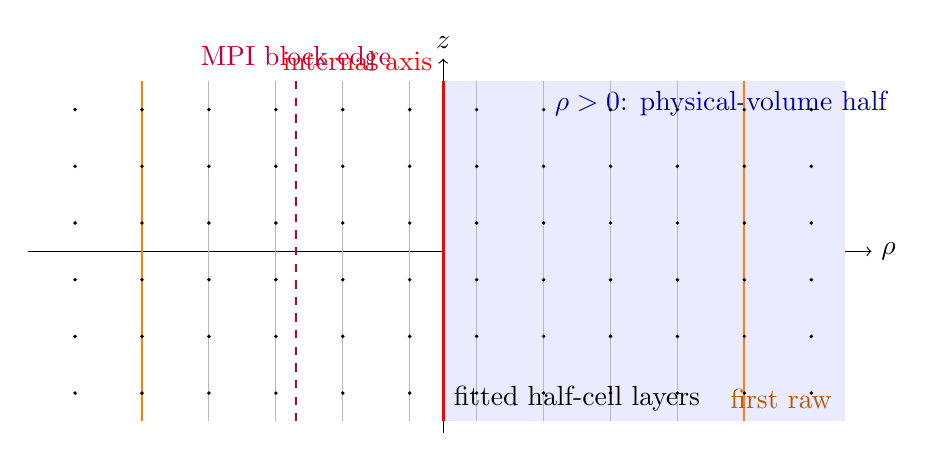
\begin{tikzpicture}[x=0.85cm,y=0.72cm]
  \draw[->] (-6.2,0) -- (6.4,0) node[right] {$\rho$};
  \draw[->] (0,-3.2) -- (0,3.4) node[above] {$z$};
  \fill[blue!8] (0,-3) rectangle (6,3);
  \node[blue!60!black] at (4.15,2.6) {$\rho>0$: physical-volume half};
  \draw[very thick,red] (0,-3) -- (0,3) node[above left] {internal axis};
  \foreach \x in {-3.5,-2.5,-1.5,-.5,.5,1.5,2.5,3.5}
    \draw[gray!55] (\x,-3) -- (\x,3);
  \draw[orange,thick] (-4.5,-3) -- (-4.5,3);
  \draw[orange,thick] (4.5,-3) -- (4.5,3);
  \node[orange!70!black] at (5.05,-2.6) {first raw};
  \node at (2.0,-2.6) {fitted half-cell layers};
  \draw[dashed,thick,purple] (-2.2,-3) -- (-2.2,3)
    node[above,purple] {MPI block edge};
  \foreach \x in {-5.5,-4.5,...,5.5}
    \foreach \y in {-2.5,-1.5,...,2.5} \fill (\x,\y) circle (0.7pt);
\end{tikzpicture}
\else
\setlength{\unitlength}{0.55cm}
\begin{picture}(22,12)(-11,-6)
  \put(-10,0){\vector(1,0){20}} \put(10.3,-0.2){$\rho$}
  \put(0,-5){\vector(0,1){10}} \put(0.2,5.1){$z$}
  \put(0,-5){\line(0,1){10}} \put(-2.4,4.2){internal axis}
  \put(1,-4.5){$\rho>0$: physical-volume half}
  \put(4,-5){\line(0,1){10}} \put(4.2,-4.5){first raw}
  \put(-5,-5){\line(0,1){10}} \put(-8.8,4.2){MPI block edge}
  \multiput(-9,-4)(2,0){10}{\circle*{0.12}}
  \multiput(-9,-2)(2,0){10}{\circle*{0.12}}
  \multiput(-9,0)(2,0){10}{\circle*{0.12}}
  \multiput(-9,2)(2,0){10}{\circle*{0.12}}
  \multiput(-9,4)(2,0){10}{\circle*{0.12}}
\end{picture}
\fi
\caption{Real $n_3=1$ cell-centered signed plane.  No active half-cell is relabeled
as $\rho=0$; exact-axis checks use a separate bounded axis-centered provider view.}
\end{figure}

\subsection{Operator and norm contract}
\begin{center}
\begin{tabular}{lr}
\toprule
Family & independent runtime series\\
\midrule
scalar: first, symmetric second, advection & 10\\
vector: three components plus divergence & 31\\
tensor all-lower & 60\\
tensor all-upper & 60\\
component dissipation & 10\\
\midrule
Total & 171\\
\bottomrule
\end{tabular}
\end{center}
Uniform norms use every owned active cell exactly once.  Cylindrical norms use only
$\rho>0$ with measure $2\pi\rho\,d\rho\,dz$.  The first raw strip gives the mixed
global expectations $p$, $p-1/2$, and $p-1$ in uniform $L_1,L_2,L_\infty$;
region-filtered regular and fitted series own the formal $p$ gates, while the first
raw layer owns $p-1$.  Fixed signed targets record both requested and actual sampled
radii.
Explicitly, for owned-cell errors $e_i$,
\[
 L_1={1\over n}\sum_i|e_i|,\quad
 L_2=\left({1\over n}\sum_i e_i^2\right)^{1/2},\quad
 L_\infty=\max_i|e_i|,
\]
while $L_{1,\rm cyl}=\sum_{\rho_i>0}w_i|e_i|/\sum w_i$,
$L_{2,\rm cyl}=(\sum w_ie_i^2/\sum w_i)^{1/2}$, and
$L_{\infty,\rm cyl}=\max_{\rho_i>0}|e_i|$, with
$w_i=2\pi\rho_i\Delta\rho\Delta z$.  Signed masks separately retain regular
$|\rho|\ge0.75$, each fitted half-cell layer, the first raw layer, and the
requested/actual $|\rho|=0.5$ probes.  Negative-only masks deliberately have no
cylindrical statistic.

The 171-name generated manifest classifies 149 truncating series, 12 exact-zero
SO(2) identities, and 10 exact-discrete dissipation comparisons.  Only truncating
series receive rate gates; exact classes receive finite/presence and frozen absolute
bounds.  The full-plane uniform expectations are respectively $p,p-1/2,p-1$ for
$L_1,L_2,L_\infty$; cylindrical $L_1,L_2$ expect $p$ and cylindrical $L_\infty$
expects $p-1$.  Region-filtered regular/fitted masks expect $p$, and the raw mask
expects $p-1$.

\subsection{Controlled perturbations}
Let $\ell$ be the absolute radial layer, $j$ the axial index, $c$ a component
index, and $q\in[0,7]$ the phase.  The deterministic pattern is
\[
 \eta_{\ell jcq}={((17\ell+13j+7q+5c+3c^2)\bmod23)-11\over11},
 \qquad a=(2\ \hbox{float or }64\ \hbox{double})\,\epsilon_{\rm Real}.
\]
The shared-parity lane adds $a\eta$ to the scalar,
$a(\rho\eta,\eta,\rho\eta)$ to the vector, and
$a((1+\rho^2)\eta,\rho\eta,\rho^2\eta,\eta,-\rho\eta,
(1-\rho^2)\eta)$ to the six tensor components.  The independent lane leaves
scalar/vector data clean and adds separately indexed even patterns only to
$T_{\rho\rho},T_{\rho Y},T_{YY}$.  Every record carries both noisy error-to-oracle
and the direct noisy-minus-clean result.  The generated series manifest states the
affected lane of each result; saturation is declared before rate fitting from the
direct delta, never after observing a disappointing rate.

\subsection{Implementation and dispatch}
The thin input-selected pgen is non-templated.  It passes one opaque host context to
the separately compiled \texttt{DispatchCartoonZ4cKernel} seam, which selects exactly
one of the order-2/4/6 entry points before any Kokkos launch.  Device kernels capture
only the concrete \texttt{CartoonSO2,NGHOST} provider; there is no per-cell symmetry
or order branch.  The clean manufactured field occupies the real
\texttt{pz4c->u0} view with extent $n_3=1$; two collapsed scratch views hold the
noise lanes.  The pgen restores a Minkowski sentinel and asserts cycle and time are
unchanged before returning.  Cartesian provider and generated finite-difference
sources remain checksum-frozen.

\subsection{Qualification records}
The immutable driver requires $N=32,64,128,256$, all eight deterministic noise
phases, orders $2,4,6$, CPU MPI sizes two and four, and CUDA MPI size four with four
distinct A100 UUIDs.  It rejects missing/nonfinite series, ownership sequences other
than $[0,N^2)$, backend fallback, partial case directories, and mismatched hashes.

\IfFileExists{data/index.tex}{%
\ifmmsplots
\input{data/index}
\else
\PackageError{cartoon-mms}{Reviewed data require tikz and pgfplots}{Install the
required TeX packages; numerical plots may not be silently omitted.}
\fi
}{%
\begin{center}\fbox{\parbox{0.82\linewidth}{Fresh reviewed backend data are not
yet present.  This is an explicit evidence boundary, not a numerical result.}}\end{center}
}

Final acceptance must add source/tree/submodule and executable hashes, compiler and
Kokkos identities, per-translation-unit wall/RSS evidence, CPU rank comparison,
CUDA UUID binding, saturation classifications, failures, and data-linked plots.

\subsection{Exact build and runtime interface}
Both routine builds target only \texttt{athena}, with the built-in pgen dispatcher,
MPI enabled, OpenMP disabled, unit tests disabled, Release mode, and parallelism
eight.  The CPU cache requires Kokkos Serial on/CUDA off.  The CUDA cache requires
\texttt{cc}/\texttt{CC}, CUDA lambda/constexpr, Serial off, and Ampere80.  The
checksum-bound campaign command is
\begin{quote}\ttfamily
python3 tst/test\_suite/unit\_tests/test\_z4c\_cartoon\_derivatives.py
--athena /path/to/athena --launcher ``srun'' --ranks 4
--output /path/to/evidence
\end{quote}
with the checked-in input, exact orders $2,4,6$, resolutions
$32,64,128,256$, and phases $0,\ldots,7$ supplied by default and enforced.  CPU
qualification runs the same executable at two and four ranks and compares clean,
shared, independent, direct-delta, probe, ownership, and binding inventories.  CUDA
qualification requires four rank-local, distinct A100 UUID records.  Build/runtime
results remain pending independent Perlmutter execution; the present PDF records
source-review structure only.

\subsection{Frozen legacy-check ownership}
\begin{longtable}{p{0.43\linewidth}p{0.48\linewidth}}
\toprule ID & owner\\\midrule
LEG-PARITY-METADATA; LEG-MINIMAL-FIT-REACH-NG2/3/4;
LEG-BLOCK-EDGE-REACH-NG2/3/4; LEG-VARIANCE-INSTANTIATION &
ordinary lightweight structural executable\\
LEG-PI-ROTATION; LEG-NOISE-DELTA; LEG-SAMPLE-RESULT-SPACE;
LEG-FULL-CARTOON-API; LEG-FIXED-RAW-POS/NEG-NG2/3/4;
LEG-REGULAR-CONV-NG2/3/4; LEG-FITTED-RAW-CONV-NG2/3/4;
LEG-SHARED-PARITY-NOISE-NG2/3/4;
LEG-INDEPENDENT-TENSOR-NOISE-NG2/3/4;
LEG-DIAGNOSTIC-AXIS-NG2/3/4 & immutable production campaign driver\\
LEG-CARTESIAN-DELEGATION; LEG-DISS-EXACTLY-ONCE-NG2/3/4 & static source/hash gate\\
LEG-FIELD-JET-ORACLE; LEG-DISS-ORACLE; LEG-ORDER-AGGREGATION-NG2/3/4 &
explicit low-frequency split standalone\\\bottomrule
\end{longtable}
